\svnkwsave{$RepoFile: siminos/spatiotemp/chapter/Kolmogorov.tex $}
\svnidlong {$HeadURL: svn://zero.physics.gatech.edu/siminos/spatiotemp/chapter/Kolmogorov.tex $}
{$LastChangedDate: 2019-05-09 18:30:52 -0400 (Thu, 09 May 2019) $}
{$LastChangedRevision: 6822 $} {$LastChangedBy: predrag $}
\svnid{$Id: Kolmogorov.tex 6822 2019-03-29 16:04:23Z predrag $}

\chapter{Kolmogorov flow}
\label{chap:Kolmogorov}
% Predrag                                            7 Dec 2018

\begin{description}

\PCpost{2018-12-07}{
% Predrag moved  to here      7 Dec 2018

Moved \emph{elton/blog/KFsymm.tex}  Mohammad and Predrag 2D Kolmogorov flow
discussions to here, current \refsect{sect:KFsymm}.
}

\MNGpost{2018-12-07}{
Mhm
}

\end{description}

%      extracted from blogMNG.tex

\svnkwsave{$RepoFile: siminos/spatiotemp/chapter/KFsymm.tex $}
\svnidlong {$HeadURL: svn://zero.physics.gatech.edu/siminos/spatiotemp/chapter/KFsymm.tex $}
{$LastChangedDate: 2019-05-09 18:30:52 -0400 (Thu, 09 May 2019) $}
{$LastChangedRevision: 6822 $} {$LastChangedBy: predrag $}
\svnid{$Id: KFsymm.tex 6822 2019-03-29 16:04:23Z predrag $}


\section{Notes on Kolmogorov flow}
\label{sect:KFsymm} % was \label{s:KFlit}
% Predrag moved elton/blog/KFsymm.tex  to here      7 Dec 2018

\begin{description}


\MFpost{2017-07-10}{
Read
\HREF{http://bura.brunel.ac.uk/handle/2438/14877}
{Smith and Wissink}\rf{SmiWis17} {\em Asymptotic analysis of the
attractors in two-dimensional Kolmogorov flow}.
}

%\PCpost{2017-07-10}{
%%\begin{verbatim}
%Mohammad Farazmand	mfarazmand7 	No2grandmothers
%%\end{verbatim}
%}

{\bf 2015-06-24 Predrag}
I was careless. Looks much simpler than \Dn{4}.
The generator \LieEl\ of the vertical \emph{cyclic symmetry group}
$\Zn{2n}=\{e,\LieEl,\LieEl^2,\cdots,\LieEl^{2n-1}\}$
of order $2n$ is a \emph{glide reflection}\rf{PlSiFi91}
\beq
\LieEl \, \bu(x,y)=
\begin{pmatrix}
- u(-x,y+\pi/n)\\
v(-x,y+\pi/n)
\end{pmatrix}
\,,
\ee{GlideRefl}
All $2n$ irreps are 1\dmn, with characters $\chi(g^{k}) = \omega^k$,
$\omega=\exp(\pi/n)$.
For $n=4$ the 8 irreps Frobenius character projection
operators \refeq{irrepFncts} are the discrete Fourier transforms
\bea
% && \qquad\qquad\qquad\qquad\qquad\qquad
%              ~~~~~~ \trHalf{x} ~~\, \trHalf{z}    ~\, \trHalf{xz}
%    \continue
\beUBg{1} &=& \frac{c_{1}}{8}
              (1 + \omega^{-1} \LieEl + \omega^{-2}\LieEl^2 + \cdots + \omega^{1}\LieEl^{2n-1})
      \, \uEQ      %~~~~  +  ~~  +     ~~   +
    \continue
\beUBg{2} &=& \frac{c_{2}}{8}
              (1 + \omega^{-2} \LieEl^2 + \omega^{-4}\LieEl^4 + \cdots + \omega^{2}\LieEl^{2n-2})
      \, \uEQ      %~~~~  +  ~~  -     ~~
    \label{globalKFframe}\\
\beUBg{3} &=& \frac{c_{1}}{8}
              (1 + \omega^{-3}  \LieEl^3 + \omega^{-6}\LieEl^6 + \cdots )
      \, \uEQ      %~~~~  -  ~~  +     ~~   - - 4n-2 2n + 2(n-1)
     \continue
\beUBg{2n-1} &=& \frac{c_{2}}{8}
              (1  + \omega\LieEl^{2n-1} + \cdots)
      \, \uEQ      %~~~~  -  ~~  -     ~~   +
    \nnu
\,,
\eea
The invariant subgroups are the cyclic groups $\{e\}$,
$\Zn{2} = \{e,\LieEl^4\}$ (translations by $\pi$),
$\Zn{4} = \{e,\LieEl^2,\LieEl^4,\LieEl^6\}$ (translations by $\pi/2$),
and \Zn{8}.

Aside: Should also understand first the relation between a fundamental domain for
\Zn{3} (3-disk in magnetic field) and these complex eigenvectors.

However, the rotation
\beq
R\,\bu = [-u(-x,-y),-v(-x,-y)]
\ee{KFrot}
does not commute with vertical \Zn{2n},
    \PC{2015-06-24}{please recheck}
\[
R \LieEl\,\bu = R [-u(-x,y+\pi/4),v(-x,y+\pi/4)]
         = [ u( x,-y-\pi/4),-v(x,-y-\pi/4)]
\]
\[
\LieEl R\,\bu = \LieEl [-u(-x,-y),-v(-x,-y)]
         = [ u( x,-y+\pi/4),-v(x,-y+\pi/4)]
\,,
\]
so the full order 16 group is more complicated than $\Zn{8}\times \Zn{2}$
(for possible groups \HREF{http://groupprops.subwiki.org/wiki/Groups_of_order_16}{click here}).
Instead, we have
\[
\LieEl^{-1} R\,\bu = \LieEl [-u(-x,-y),-v(-x,-y)]
         = [ u( x,-y-\pi/4),-v(x,-y-\pi/4)]
\,,
\]
so the generator algebra is of \Dn{8}:
\beq
R^2=e       \,,\quad
\LieEl^8=e \,,\quad
R \LieEl = \LieEl^{-1} R
\,.
\ee{D8gen}
%}

A presentation of \Dn{n} is
\beq
\langle \LieEl, R\mid \LieEl^n = R^2 = e, R\LieEl=\LieEl^{-1}R \rangle
\ee{presentDn}

%%%%%%%%%%%%%%%%%%%%%%%%%%%%%%%%%%%%%%%%%%%%%%%%%%%%%%%%%%%%%%%%%%%%%%
% PC 2015-06-20 adopted from siminos/xiong/thesis/chapters/symm.tex
\paragraph{Dihedral group $\Dn{8}$.}
\label{exam:D8chars}
The  \Dn{8} group
\[\Dn{8}=\{e,\LieEl,\LieEl^2,\LieEl^3,\cdots,\LieEl^7,
           R,R\LieEl^2,R\LieEl^3,\cdots,R\LieEl^7 \}
\]
has a
$8$ shift elements and $8$ shift-reflect elements.
There are $7$ classes:
$\{e\}$,
$\{\LieEl^4\}$,
$\{\LieEl^2,\LieEl^6\}$,
$\{R,R\LieEl^4\}$ and
$\{R\LieEl^2,R\LieEl{3/4}\}$.
There are four different one-dimensional irreducible representations,
whose characters are $\pm 1$ under reflection $R$ and shift-reflect
operation $R\LieEl$.
There are three 2-dimensional representations $E_j$.
It has 3 subgroups:  \Zn{4},  \Dn{2} and  \Zn{2}.
Life can be made easier by defining the quarter-shift as
$\LieEl{} = \LieEl$,
with $R^2=e$, $\LieEl^8=e$, and
$R\LieEl=\LieEl^{-1}R$.
The character table is given in \reftab{tab:D8char}.
    \PC{2015-06-25,2019-03-29}{\refTab{tab:D8char} not completed yet;
    needs 2 more E irreps to get the sum of (dim)$^2$ to 16. I started with
    Xiong's thesis \Dn{n}, not yet cross-checked with tables on the web.
    }
%%%%%%%%%%%%%%%%%%%%%%%%%%%%%%%%%%%%%%%%%%%%%%%%%%%%%%%%%%%%%%%%%%%%%%

%%%%%%%%%%%%%%%%%%%%%%%%%%%%%%%%%%%%%%%%%%%%%%%%%%%%%%%%%%%%%%%%%%%%%%
% PC 2015-06-25 adopted from siminos/xiong/thesis/chapters/symm.tex
\begin{table}
\begin{center}
\begin{tabular}{c|ccccccc}
$\Dn{8}$       & $A_1$& $A_2$& $B_1$& $B_2$& $E_1$ & $E_2$ & $E_3$\\
\hline
$\{e\}$        &   1  &   1  &  1   &  1  &  2  &  2  &  2  \\
$\{\LieEl^{2}\}$
               &   1  &   1  &  1   &  1  & -2 \\
$\{\LieEl{},\LieEl^{-1}\}$
               &   1  &   1  & -1   & -1  &  0  \\
$\{R,R\LieEl^{2}\}$
               &   1  &  -1  &  1   & -1  &  0  \\
$\{R\LieEl{},R\LieEl^{-1}\}$
               &   1  &  -1  &  -1  & 1   &  0   \\
$\{\LieEl{}^2,\LieEl^{-2}\}$
               &   ?  &   ?  & -?   & -?  &  ?  \\

$\{\LieEl{}^3,\LieEl^{-3}\}$
               &   ?  &   ?  & -?   & -?  &  ?  \\
\end{tabular}
\end{center}
  \caption{\label{tab:D8char}
Character table of dihedral group $\Dn{8}$.
  }
\end{table}
%%%%%%%%%%%%%%%%%%%%%%%%%%%%%%%%%%%%%%%%%%%%%%%%%%%%%%%%%%%%%%%%%%%%%%%


\MFpost{2015-06-24}{Lets define
\begin{equation}
(\tau\mathbf u)(x_1,x_2)=
\begin{pmatrix}
u_1(x_1,x_2+\pi/2)\\
u_2(x_1,x_2+\pi/2)
\end{pmatrix},
\end{equation}
and
\begin{equation}
(\sigma\mathbf u)(x_1,x_2)=
\begin{pmatrix}
-u_1(-x_1,x_2+\pi/4)\\
\quad u_2(-x_1,x_2+\pi/4)
\end{pmatrix}.
\end{equation}

Then all elements of the glide reflection symmetry can be written as
\[\Dn{4}=\{e,\trDiscr{}{1/4},\trDiscr{}{1/2},\trDiscr{}{3/4},
           \sigma,\sigma\trDiscr{}{1/4},
           \sigma\trDiscr{}{1/2},\sigma\trDiscr{}{3/4} \}.
\]
However,
$$\sigma\tau\neq \tau^{-1}\sigma, \quad \sigma^2\neq e.$$
Instead we have
$$\sigma\tau= \tau\sigma,\quad \sigma^2=\tau.$$
Do formulas \eqref{globalUBframe} still work?
\\
{\bf 2015-07-07} Now need sum over 16 elements, otherwise the same.
}

\PCpost{2015-06-21}{
Reading Platt, Sirovich, and Fitzmaurice\rf{PlSiFi91}:

For {Kolmogorov} flow they credit
V. I. Arnold and L. D. Meshalkin, Usp. Mat. Nauk 15, 247 (1960),
an article that I have not had a look at.

Stability was studied in the above article, as well as by Green\rf{Green74}.
Green studies various stable solutions, and does not cite Kolmogorov.

A stationary cellular
pattern that appears beyond the first bifurcation was discussed
G. I. Sivashinsky, Physica D 17, 243 (1985).

G. I. Sivashinsky and V. Yakhot, Phys. Fluids 28, 1040 (1985);
V. Yakhot and G. I. Sivashinsky, Phys. Rev. A 35, 815 ( 1987)
interpret long-wavelength instabilities as `negative viscosity'.

One needs to also look at
N. F. Bondarenko,. M. Z. Gak, and F. V. Dolzhansky, Atmos. Ocean.
Phys. 15, 711 (1979).

This system has \eqv\ solution
\beq
u(x,y)=\frac{Re}{n^2}\sin(n y),\quad v(x,y)=0,
\ee{KFeqv0blog}
A Reynolds number $\Reynolds$ for the flow may be naturally based on the
maximum speed of this solution, and the forcing length scale. This \eqv\
goes unstable at $\Reynolds=n\sqrt{2}$. Sufficiently high wavenumber
eigenvectors are always stable. They define doubly-periodic rectangular
domain
\[
(x,y)\in [0,2\pi]\times [0,2\pi]
\]
They use a spectral basis that is automatically divergence free,
and compute for the $n = 4$ case.
All runs are initiated as random perturbations off the ustable \eqv\
\refeq{KFeqv0blog}. 5000 + time units were integrated before
before any data were recorded.
[$16 \times 16$] spatial grid gave rise to underresolved
flows that were drastically different in nature, so their computations are
for [$32 \times 32$]  (i.e., 1024 ordinary differential equations).
This was
found adequate for the parameter range
$\Omega/\Omega_c<12.5$.

A stable \reqv\ bifurcates of an \eqv\ up at $\Omega/\Omega_c = 2.2$,
with phase velocity starting with 0.

For $1.97<\Omega/\Omega_c<2.2$ one is in regime where stable \eqv\ with
horizontal $\Zn{2}$ (or $\Dn{2}$ or some other symmetry?) rules.
This symmetry is also noted by Green\rf{Green74}. Apparently all stable
equilibria up to and including this one are invariant under the full
16-element discrete symmetries.

They find it remarkable that narrow stability windows in $\Omega/\Omega_c$
appear interspersed between chaotic episodes. Looks sensible to me.

Of all the chaotic states they observed, fig.~14 is the only state that
they dare
chaotic both spatially and temporally and hence
turbulent, according to common convention.



Their Kaplan-Yorke (`Lyapunov') dimension is accurate to the first digit only.
By the time they get to $\Omega/\Omega_c=12.5$ it is about 11.

\emph{Poincar\'e sections} were computed following Keefe\rf{Keefe85}. They
realize that the Poincar\'e section planes should be invariant under the
symmetry (both discrete and continuous). They find it a good practice to
choose as a section a plane for which the flow projections maximize the
energy with respect to the L2 norm.

Their \emph{discussion of symmetries} is clear and succinct. Will have
to use all of it.
The generator
of the vertical cyclic symmetry group of order $2n$ is a \emph{glide reflection}
(here eq.~(13)). In eqs.~(31), (32)
they give explicit action of symmetries on the Fourier basis.

Rotation through $\pi$ in is another group
generator, i.e., if $\bu$ is a Kolmogorov flow then
\[
R \bu \to [-u(-x,-y),-v(-x,-y)]
\]
is one also. In all there are $4n$ discrete symmetries group elements.

The remaining symmetry group is the continuous group of translations
in the $x$ direction.

    }

\PCpost{2015-06-24}{
Even though Sirovich\rf{Sirovich87} cites Birkhoff and
MacLane\rf{BirkMacL63} for \emph{glide reflection}, I did not find it in
that book. However, glide reflection is standard, described many
places.
%http://www.math.uchicago.edu/~may/VIGRE/VIGRE2008/REUPapers/Levine.pdf
Perhaps these would be good references, if a citation is needed (I have
not looked at them):

\noindent
H.S.M. Coxeter. Introduction to Geometry. John Wiley and Sons, Inc. 1969.
\\
Heinrich W. Guggenheimer. Plane Geometry and its Groups. Holden-Day. 1967.
\\
Killingbeck\rf{Killingbeck70} might be
a potentially useful reference (maybe too chemical?)

There are four isometries in the plane: translation, rotation,
reflection, and glide reflection, see \reffig{fig:BaloglouSketch}.
A \emph{reflection} flips points over an invariant axis or line. A
\emph{glide reflection} combines a reflection with a translation along
the direction of the mirror line.

%%%%%%%%%%%%%%%%%%%%%%%%%%%%%%%%%%%%%%%%%%%%%%%%%%%%%%%%%%%%%%%%%%%%
% http://www.emis.de/monographs/Isometrica/circle-isometries.pdf
\begin{figure}
  \centering
  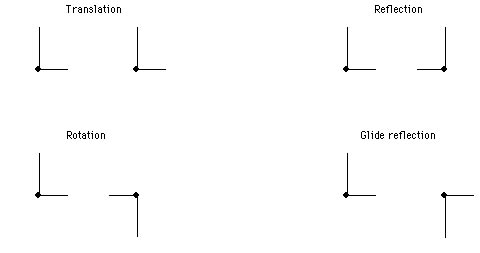
\includegraphics[width=0.40\textwidth]{BaloglouSketch}
  \caption{
The four isometries in the plane.
  }\label{fig:BaloglouSketch}
\end{figure}
%%%%%%%%%%%%%%%%%%%%%%%%%%%%%%%%%%%%%%%%%%%%%%%%%%%%%%%%%%%%%%%%%%%%

Glide reflections commute with each other, which is not generally the
case for any two given isometries. Given two
congruent sets on the plane, it is in general either a rotation or a
glide reflection -- depending on the orientation between them -- that
maps one to the other. Reflections and non-trivial glide reflections are
mutually exclusive.

The isometry group of a polygon may only consist of rotations and
reflections. In fact only 2 types of such groups are possible, the cyclic
groups \Zn{n} and the dihedral groups \Dn{n} (Leonardo (da Vinci)'s Theorem).
Translations and glide reflections may leave an infinite set invariant
(and presumably a finite set defined on a periodic domain),
see for example \reffig{fig:Baloglou2reflGlides}, taken from notes by
George Baloglou.

%%%%%%%%%%%%%%%%%%%%%%%%%%%%%%%%%%%%%%%%%%%%%%%%%%%%%%%%%%%%%%%%%%%%
% http://www.emis.de/monographs/Isometrica/circle-isometries.pdf
\begin{figure}
  \centering
  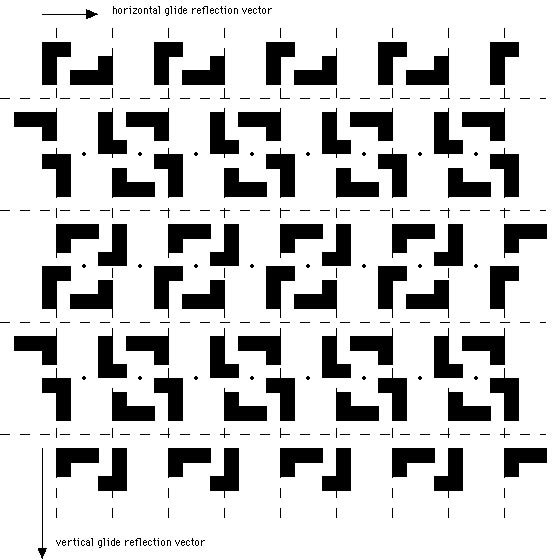
\includegraphics[width=0.40\textwidth]{Baloglou2reflGlides}
  \caption{
A wallpaper pattern of pgg type,
invariant under glide reflections (represented by dotted
lines) in two perpendicular directions.
  }\label{fig:Baloglou2reflGlides}
\end{figure}
%%%%%%%%%%%%%%%%%%%%%%%%%%%%%%%%%%%%%%%%%%%%%%%%%%%%%%%%%%%%%%%%%%%%


The lattice unit is always a \emph{generating region}, but a generating
region (fundamental domains) may be smaller than the lattice units.
    }

\PCpost{2015-06-21}{
In \refref{Sirovich87}, Sirovich discusses how to incorporate
symmetries of flows in computation of a correlation matrix from data,
for
\begin{itemize}
  \item Plane Poiseuille (channel) flow
  \item Poiseuille flow in a rectangular channel
  \item B\'enard problem (convection).
  \item Flow past bodies of revolution
  \item Flow in a circular pipe
  \item Plane Couette flow
  \item Taylor-Couette flow
  \item Flow past a circular cylinder
\end{itemize}
However, he does not mention {Kolmogorov} flow.


V. I. Arnold\rf{arnold91k}

Chandler, Lucas \&\ Kerswell\rf{ChaKer12,LucKer12,LucKer14}

R. Mitchell \rf{MitchellThesis13} PhD thesis
(in \texttt{ChaosBook.org/library}),
{\em Transition to turbulence and mixing in a quasi-two-dimensional
        {Lorentz} force-driven {Kolmogorov} flow}.
    }

\PCpost{2012-11-07 }{
In systems with continuous symmetries there are important classes of
invariant solutions referred to as `relative' or
`equivariant'\rf{Huyg1673,Poinc1896}.
                    }

\end{description}



\section{Symmetries and isotropy subgroups}
\label{s:KFsymm}
% n00bs.tex
% 2009-06-16 , 16 Jun 2009

\renewcommand{\ssp}{a}


On an infinite domain and in the absence of boundary conditions, the Navier-Stokes
equations are equivariant under any $2D$~translation, $2D$~rotation, and
$\bx \to -\bx$, $\bu \to -\bu$ inversion through the origin\rf{frisch}.
In $2D$ the inversion is the same as rotation by $\pi$.
In Kolmogorov flow, the parallel side walls restrict the rotation
symmetry to rotation by $\pi$ about the $z$-axis. We denote this rotation
by $\sigma_{x}$ and the inversion through the origin by $\sigma_{xy}$.
{The suffixes indicate
which of the homogeneous directions $x,z$ change sign and simplify the
notation for the group algebra of rotation, inversion, and translations
presented in \refsects{s:flipnshift}{s:67-fold}.}
The $\sigma_{xy}$ and $\sigma_x$ symmetries generate a discrete dihedral group
$D_1 \times D_1 = \{e,\sigma_x,\sigma_{z},\sigma_{xy}\}$ of order 4, where
\begin{align}
\sigma_x    \, [u,v](x,y) &= [-u,-v,w](-x,-y,z) \nnu \\
\sigma_y    \, [u,v](x,y) &= [u, v,-w](x,y,-z)  \label{sigma}\\
\sigma_{xy} \, [u,v](x,y) &= [-u,-v](-x,-y) \nnu
\,.
\end{align}

The walls also restrict the translation symmetry to $1D$ streamwise
translations. With periodic boundary condition, these translations
become the $\SOn{2}$ continuous one-parameter
group of streamwise translations
\begin{align}
\tau(\shift) [u,v](x,y) &= [u, v](x+\shift, y)
\,.
\label{translation}
\end{align}
The equations of Kolmogorov flow are thus equivariant under the group
$\GPKF = \On{2} \times \Dn{4} = D_{1,x} \ltimes \SOn{2} \times \Dn{4}$,
where $\ltimes$ stands for a semi-direct product, and sign changes in
$x$, and $y$ subscripts indicate spanwise translations and sign changes
in $y$.

The solutions of an equivariant system can satisfy all of the system's
symmetries, a proper subgroup of them, or have no symmetry at all. For a
given solution $\bu$, the subgroup that contains all symmetries that fix
$\bu$ (that satisfy $s \bu = \bu$) is called the isotropy (or stabilizer)
subgroup of $\bu$. \rf{hoyll06,MarRat99, golubitsky2002sp, GL-Gil07b}.
For example, a typical turbulent trajectory $\bu(\bx,t)$ has no symmetry
beyond the identity, so its isotropy group is $\{e\}$. At the other
extreme is the laminar {\eqv}, whose isotropy group is the full
Kolmogorov symmetry group $\GPKF$.

In between, the isotropy subgroup  of most
of the \eqva\ reported here is $S = \{e, s_1, s_2, s_3\}$, where
\begin{align}
s_1 \, [u,v](x,y) &= [u, v, -w](x+L_x/2, y, -z) \nnu \\
s_2 \, [u,v](x,y) &= [-u, -v, w](-x+L_x/2,-y,z+L_y/2) \label{shiftRot}\\
s_3 \, [u,v](x,y) &= [-u,-v,-w](-x, -y, -z+L_y/2) \nnu
\,.
\end{align}
Flow-invariant subgroups might play an important role in the turbulent
dynamics. In this section we provide a partial classification of the
isotropy groups of $\GPKF$, sufficient to classify all currently known
invariant solutions and to guide the search for new solutions with other
symmetries.


\subsection{Flips and half-shifts}
\label{s:flipnshift}

A few observations will be useful in what follows. First, we note the
key role played by the {rotation and reflection} symmetries $\sigma_x$
and $\sigma_y$ \refeq{sigma} in the classification of solutions and
their isotropy groups. The equivariance of Kolmogorov flow under
continuous translations allows for {\reqva} solutions, \ie,
solutions that are steady in a frame moving with a constant velocity
in $(x)$. In {\statesp}, {\reqva} either trace out
circles or wind around tori, and these sets are both
continuous-translation and time invariant. The sign changes under
$\sigma_x$ and $\sigma_{y}$, however, imply particular
centers of symmetry in $x$ and $y$,
and thus fix the translational phase of fields that are fixed by these
symmetries. Thus the presence of $\sigma_x$ or $\sigma_y$ in an
isotropy group prohibits {\reqva} in $x$ or $z$, and the
presence of $\sigma_{xy}$ prohibits any form of {\reqv}. Guided
by this observation, we will seek {\eqva} only for isotropy subgroups
that contain the $\sigma_{xy}$ inversion symmetry.

Second, the periodic boundary conditions impose discrete
translation symmetries of $\tau(L_x, 0)$ and $\tau(0, L_y)$ on
velocity fields. In addition to this full-period translation symmetry,
a solution can also be fixed under a rational translation, such as
$\tau(m L_x/n, 0)$ or a continuous translation $\tau(\ell)$.
If a field is fixed under continuous translation, it is
constant along the given spatial variable. If it is fixed under rational
translation $\tau(m L_x/n, 0)$, it is fixed under $\tau(m L_x/n,
0)$ for $m \in [1, n-1]$ as well, provided that $m$ and $n$ are
relatively prime. For this reason the subgroups of the
continuous translation $\SOn{2}$ consist of the discrete cyclic groups
$\Zn{n}$ for $n=2,3,4,\ldots$ together with the trivial subgroup $\{e\}$
and the full group $\SOn{2}$ itself. For rational
shifts $\ell_x/L_x = m/n$ we simplify the notation a bit by rewriting
\refeq{translation} as
\begin{align}
\trDiscr{x}{m/n} = \tau(m L_x/n, 0)
\,.
\label{translDisc}
\end{align}
Since $m/n = 1/2$ will loom large in what follows, we omit exponents of $1/2$:
\beq
    \trHalf{x} = \trDiscr{x}{1/2}
    \,,\;
    \trHalf{z} = \trDiscr{z}{1/2}
    \,,\;
    \trHalf{xz} = \trHalf{x} \trHalf{z}
\,.
\label{tauHalf}
\eeq
If a field $\bu$ is fixed under a rational shift $\tau(L_x/n)$,
it is periodic on the smaller spatial domain $x \in [0,L_x/n]$.
For this reason we can exclude from our searches all \eqv\
whose isotropy subgroups contain
rational translations in favor of \eqva\ computed on smaller domains.
However, as we need to study bifurcations into
states with wavelengths longer than the initial state,
the linear stability computations
need to be carried out in the full $[L_x,2]$ cell.
For example, if \tEQ{}\ is an \eqv\ solution in the
$\bCell_{1/3}= [L_x/3,2]$ cell, we refer to the
same solution repeated thrice in $\bCell = [L_x,2]$
as ``streamwise-tripled'' or
$3 \times \tEQ{}$. Such solution is by construction fixed under the
$\Zn{3} = \{e,\trDiscr{x}{1/3},\trDiscr{x}{2/3}\}$ subgroup.


Third, some isotropy groups are conjugate to each other under symmetries
of the full group $\GPKF$. Subgroup $H'$ is conjugate to $H$ if there is
an $s \in \GPKF$ for which $H' = s^{-1} H s$. In spatial terms, two
conjugate isotropy groups are equivalent to each other under a coordinate
transformation. A set of conjugate isotropy groups forms a conjugacy
class. It is necessary to consider only a single representative of each
conjugacy class; solutions belonging to conjugate isotropy groups can be
generated by applying the symmetry operation of the conjugacy.

In the present case conjugacies under spatial translation symmetries are
particularly important. Note that $\On{2}$ is not an abelian group, since
reflections $\sigma$ and translations $\tau$ along the same axis do not
commute \rf{Harter93}. Instead we have $\sigma \tau  = \tau^{-1} \sigma$.
Rewriting this relation as $\sigma \tau^{2} = \tau^{-1} \sigma \tau$, we
note that \bea \sigma_x \tau_x(\ell_x, 0)
  &=& \tau^{-1}(\ell_x/2, 0) \, \sigma_x \, \tau(\ell_x/2, 0)
\,.
\label{origShift}
\eea
The right-hand side of \refeq{origShift} is a similarity
transformation that translates the origin of coordinate system. For
$\shift_x = L_x/2$ we have
\beq
\trDiscr{x}{-1/4} \, \sigma_{x} \, \trDiscr{x}{1/4}
        = \sigma_{x} \trHalf{x}
\label{origQuartShift}
\,,
\eeq
and similarly for the spanwise shifts / reflections. Thus for
each isotropy group containing the shift-reflect $\sigma_x \tau_x$
symmetry, there is a simpler conjugate isotropy group in which
$\sigma_x \tau_x$ is replaced by $\sigma_x$ (and similarly
for $\sigma_y \tau_y$ and $\sigma_y$). We choose as the representative
of each conjugacy class the simplest isotropy group, in which all such
reductions have been made. However, if an isotropy group contains both
$\sigma_x$ and $\sigma_x \tau_x$, it cannot be simplified this way,
since the conjugacy simply interchanges the elements.

Fourth, for $\shift_x = L_x$, we have $\trHalf{x}^{-1} \, \sigma_{x} \,
\trHalf{x} = \sigma_x \,,$ so that, in the special case of half-cell
shifts, $\sigma_x$ and $\tau_x$ commute. For the same reason, $\sigma_y$
and $\tau_y$ commute, so the order-16 isotropy subgroup \beq G = D_{1,x}
\times \Zn{2} \times D_{1,z} \times C_{2,z} \subset \GPKF
\ee{order16subgrp} is abelian.


\subsection{The 67-fold path}
\label{s:67-fold}

We now undertake a partial classification
of the lattice of isotropy subgroups of Kolmogorov flow. We focus on
isotropy groups involving at most half-cell shifts, with $\SOn{2} \times \Dn{4}$
translations restricted to order 4 subgroup of spanwise-streamwise
translations \refeq{tauHalf} of half the cell length,
\beq
T = \Zn{2}\times C_{2,z}
  =  \{e,\trHalf{x},\trHalf{z},\trHalf{xz}\}
\,. \label{tauD2} \eeq All such isotropy subgroups of $\GPKF$ are
contained in the subgroup $G$  \refeq{order16subgrp}. Within $G$, we look
for the simplest representative of each conjugacy class, as described
above.


Let us first enumerate all subgroups $\isotropyG{} \subset G$.
The subgroups can be of order
$|\isotropyG{}| = \{1,2,4,8,16\}$.
A subgroup is generated by multiplication of a set of
generator elements, with the choice of
generator elements unique up to a permutation of subgroup
elements.
A subgroup of order $|\isotropyG{}| =  2$ has only one generator,
since every group element is its own inverse. There are 15
non-identity elements in $G$ to choose from, so there are 15 subgroups
of order 2.
Subgroups of order 4 are generated by multiplication of two
group elements. There are 15 choices for the first and 14
choices for the second. However, each order-4 subgroup
can be generated by $3 \cdot 2$ different choices of generators.
For example, any two of $\tau_x, \tau_y, \tau_{xz}$ in any order
generate the same group $T$. Thus there are $(15 \cdot 14)/(3 \cdot 2) = 35$
subgroups of order 4.

Subgroups of order 8 have three generators.  There are
15 choices for the first generator, 14 for the second, and 12 for the
third. There are 12 choices for the third
generator and not  13, since if it were chosen to be the product of the
first two generators, we would get a subgroup of order 4.
Each order-8 subgroup can be generated
by $7 \cdot 6 \cdot 4$ different choices of three generators, so there are
$(15 \cdot 14 \cdot 12)/(7 \cdot 6 \cdot 4) = 15$ subgroups of order 8.
In summary: there is the group $G$ itself, of order 16,
15 subgroups of order 8, 35 of order 4, 15 of
order 2, and 1 (the identity) of order 1,
or 67 subgroups in all \rf{HalcrowThesis}.
This is whole lot of isotropy subgroups to juggle; fortunately,
the observations of \refsect{s:flipnshift} show that there
are only 5 {\em distinct conjugacy classes} in which we can expect
to find \eqva.

The 15 order-2 groups fall into 8 distinct conjugacy
classes, under conjugacies between $\sigma_x \tau_x$ and $\sigma_x$
and $\sigma_y \tau_y$ and $\sigma_y$. These conjugacy classes are
represented by the 8 isotropy groups generated individually by the 8
generators
$\sigma_x,\, \sigma_y,\, \sigma_{xy},\, \sigma_x \tau_y,\,  \sigma_y \tau_x,\,
\tau_x,\, \tau_y,\,$ and $\tau_{xz}$. Of these, the latter three imply
periodicity on smaller domains. Of the remaining five,
$\sigma_x$ and $\sigma_x \tau_y$ allow {\reqva} in $z$,
$\sigma_y$ and $\sigma_y \tau_x$ allow {\reqva} in $x$.
Only a single conjugacy class, represented by the isotropy
group
\beq
  \{e,\sigma_{xy}\}
\,,
\ee{S3subgrp}
breaks both continuous translation symmetries. Thus, of all
order-2  isotropy groups, we expect only this group to have {\eqva}.

Of the 35 subgroups of order 4, we need to identify those that
contain $\sigma_{xy}$ and thus support {\eqva}. We choose
as the simplest representative of each conjugacy class the isotropy
group in which $\sigma_{xy}$ appears in isolation.
Four isotropy subgroups of order 4 are generated by picking
$\sigma_{xy}$ as the first generator, and $\sigma_{z},\, \sigma_{z}
\trHalf{x},\, \sigma_{z} \trHalf{z},\,$ or $\sigma_{z} \trHalf{xz}$
as the second generator (\emph{R} for reflect-rotate):
\begin{align}
 R~~  &=  \{e, \sigma_x, \sigma_y, \sigma_{xy}\}
      ~~~~~~~\; = \{e,\sigma_{xy}\} \times \{e,\sigma_{z}\} \nnu\\
 R_x~ &=  \{e,\sigma_x \trHalf{x}, \sigma_y \trHalf{x}, \sigma_{xy}\}
      ~~ = \{e,\sigma_{xy}\} \times \{e,\sigma_{x}\trHalf{x}\}
        \label{subg4RR} \\
 R_y~ &=  \{e, \sigma_x \trHalf{z}, \sigma_y \trHalf{z}, \sigma_{xy}\}
      ~~\; = \{e,\sigma_{xy}\} \times \{e,\sigma_{z}\trHalf{z}\}
        \nnu\\
 R_{xz} &= \{e, \sigma_x \trHalf{xz}, \sigma_y \trHalf{xz}, \sigma_{xy}\}
        = \{e,\sigma_{xy}\} \times \{e,\sigma_{z}\trHalf{xz}\}
        \simeq S \,. \nnu
\end{align}
These are the only isotropy groups of order 4 containing $\sigma_{xy}$
and no isolated translation elements. Together with $\{e,\sigma_{xy}\}$,
these 5 isotropy subgroups represent the 5 conjugacy classes in
which expect to find {\eqva}.


\section{{\StateDsp} visualization}
\label{s:KFvisualStatSp}

\refRef{GHCW07} presents a method for visualizing low-dimensional
projections of trajectories in the infinite-dimensional {\statesp} of the
Navier-Stokes equations. Briefly, we construct an orthonormal basis
$\{\be_1, \be_2, \cdots, \be_n\}$ that spans a set of physically
important fluid states $\bu_A$, $\bu_B$, $\dots$, such as {\eqv} states
and their eigenvectors, and we project the evolving fluid state $\bu(t)$
onto this basis using the $L^2$ inner product \refeq{innerproduct}. This
produces a low-dimensional projection
\beq
\ssp(t) =(\ssp_1, \ssp_2, \cdots, \ssp_n, \cdots)(t)
    \,,\qquad
\ssp_n(t) = (\bu(t), \be_n)
\,,
\ee{intrSspTraj}
which can be viewed in $2d$ planes $\{\be_m, \be_n\}$ or in $3d$
perspective views $\{\be_{\ell},\be_m, \be_n\}$. The {\stateDsp}
portraits are {\em dynamically intrinsic}, since the projections are
defined in terms of intrinsic solutions of the equations of motion, and
{\em representation independent}. Such bases are
effective because moderate-\Reynolds\ turbulence explores a small
repertoire of unstable coherent structures, so that the trajectory $a(t)$
does not stray far from the subspace spanned by the key structures.

There is no {\em a priori} prescription for picking a `good' set of
basis fluid states, and construction of $\{\be_n\}$ set requires
some experimentation. As shown in
\refref{GHCW07}, the dynamics of different regions of {\statesp}
can be elucidated by projections onto basis sets constructed from
combinations of {\eqva} and their eigenvectors.

% ------------------------------------------------------------
% ChaosBook \Chapter{symm}{11apr2015}{Discrete symmetry factorization}

A group element $\LieEl\in \Group$ acts on  a function
$\rho(\ssp)$ defined on \statesp\ $\pS$ by its {\em operator representation}
\beq
U(\LieEl)\,\rho(\ssp) = \rho(\matrep{\LieEl}^{-1}\ssp)
\,.
\ee{ActOnFcts}
This is the conventional, Wigner definition of the effect of
transformations.

The Frobenius `character orthogonality' theory of \irrep s
(irreducible representations) of finite groups
says that all invariant
subspaces are obtained by weighted averages (`projections')
\beq
\rho^{(\irreplab)}(\ssp)
    =
\frac{d_\irreplab}{|\Group|} \sum_{\LieEl}
\character{\irreplab}{\LieEl}\,U(\LieEl)\,\rho(\ssp)
    =
\frac{d_\irreplab}{|\Group|} \sum_{\LieEl}
\character{\irreplab}{\LieEl}\,\rho(\matrep{\LieEl^{-1}}\ssp)
\ee{irrepFncts}

The simplest example is afforded by the 1\dmn\ subspace (irrep)
given by the fully symmetrized average of components of the regular basis
function $\rho^{reg}(\ssp)$
\[
\rho^{(A_1)}(\ssp)
    =
 \frac{1}{|\Group|} \sum_{\LieEl}^\Group \rho(\matrep{\LieEl}\,\ssp)
\,.
\]
By construction, $\rho^{(A_1)}$ is invariant under all actions of the group,
\(
U(\LieEl)\,\rho^{(A_1)}(\ssp) = \rho^{(A_1)}(\ssp)
 \,.
\)
This $\rho^{(A_1)}(\ssp)$ invariant subspace is a special case
of \refeq{irrepFncts},
with all $\character{A_1}{\LieEl}=1$.
In other words, for every ${\LieEl}$ this is an eigenvector of the
{\regrep} $\regmatrep{\LieEl}$ with eigenvalue 1.


By now the group acts in many different ways, so let us recapitulate:

  \begin{tabular}{r c l}
    $\LieEl~$ &~~~ & abstract group element, multiplies other elements \\[0.3em]
    $\matrep{\LieEl}$ &~~~ & [$d\!\times\!d$] \statesp\  transformation matrix,
                      multiplies $\ssp\in\pS$ \\[0.3em]
    $U(\LieEl)$ &~~~ & operator,
                acts on functions $\rho(\ssp)$ defined over \statesp\ $\pS$\\[0.3em]
    $\matirrep{\irreplab}{\LieEl}$ &~~~ & [$d_\irreplab\!\times\!d_\irreplab$]
               irrep,  acts on invariant subspace $\rho^{(\irreplab)}(\sspRed)$
  \end{tabular}

Note that the {\statesp} transformation $\matrep{\LieEl} \neq \matrep{e}$
can leave sets of `{\em boundary}' points  invariant (or `invariant
points'); for example, under reflection
$\sigma$ across a symmetry plane, the plane itself remains invariant.

%%%%%%%%%%%%%%%%%%%%%%%%%%%%%%%%%%%%%%%%%%%%%%%%%%%%%%%%%%%%%%%%%%%%%%
% PC 2015-06-20 adopted from siminos/xiong/thesis/chapters/symm.tex
\paragraph{Dihedral group $\Dn{4}$.}
\label{exam:D4chars}
The  \Dn{4} group
\[\Dn{4}=\{e,\trDiscr{}{1/4},\trDiscr{}{1/2},\trDiscr{}{3/4},
           \sigma,\sigma\trDiscr{}{1/4},
           \sigma\trDiscr{}{1/2},\sigma\trDiscr{}{3/4} \}
\]
has a
$4$ shift elements and $4$ shift-reflect elementS.
There are $5$ classes:
$\{e\}$,
$\{\trDiscr{}{1/2}\}$,
$\{\trDiscr{}{1/4},\trDiscr{}{3/4}\}$,
$\{\sigma,\sigma\trDiscr{}{1/2}\}$ and
$\{\sigma\trDiscr{}{1/4},\sigma\trDiscr{}{3/4}\}$.
There are four different one-dimensional irreducible representations,
whose characters are $\pm 1$ under reflection $\sigma$ and shift-reflect
operation $\sigma\trDiscr{}{1/4}$.
There is one 2-dimensional representation $e$.
It has 3 subgroups:  \Zn{4},  \Dn{2} and  \Zn{2}.
Life can be made easier by defining the quarter-shift as
$\trDiscr{}{} = \trDiscr{}{1/4}$,
with $\sigma^2=e$, $\trDiscr{}{4}=e$, and
$\sigma\trDiscr{}{}=\trDiscr{}{-1}\sigma$.
The character table is given in \reftab{tab:D4char}.
    \PC{2015-06-21:  I started with Xiong's thesis \Dn{n},
    cross-checked with tables on the web. Hopefully correct.
    }
%%%%%%%%%%%%%%%%%%%%%%%%%%%%%%%%%%%%%%%%%%%%%%%%%%%%%%%%%%%%%%%%%%%%%%

%%%%%%%%%%%%%%%%%%%%%%%%%%%%%%%%%%%%%%%%%%%%%%%%%%%%%%%%%%%%%%%%%%%%%%
% PC 2015-06-20 adopted from siminos/xiong/thesis/chapters/symm.tex
\begin{table}
\begin{center}
\begin{tabular}{c|ccccc}
$\Dn{4}$       & $A_1$& $A_2$& $B_1$& $B_2$& $E$ \\
\hline
$\{e\}$        &   1  &   1  &  1   &  1  &  2  \\
$\{\trDiscr{}{2}\}$
               &   1  &   1  &  1   &  1  & -2 \\
$\{\trDiscr{}{},\trDiscr{}{-1}\}$
               &   1  &   1  & -1   & -1  &  0  \\
$\{\sigma,\sigma\trDiscr{}{2}\}$
               &   1  &  -1  &  1   & -1  &  0  \\
$\{\sigma\trDiscr{}{},\sigma\trDiscr{}{-1}\}$
               &   1  &  -1  &  -1  & 1   &  0
\end{tabular}
\end{center}
  \caption{\label{tab:D4char}
Character table of dihedral group $\Dn{4}$.
  }
\end{table}
%%%%%%%%%%%%%%%%%%%%%%%%%%%%%%%%%%%%%%%%%%%%%%%%%%%%%%%%%%%%%%%%%%%%%%%


In this paper we present global views of all invariant solutions in terms
of the orthonormal `translational basis' constructed in \refref{GHCW07}
from the eight translated or translated/reflected copies of any state,
for example \uEQ, projected using the Frobenius character projection
operators \refeq{irrepFncts} on the 4 one-dimensional representations:
    \PC{2015-06-20}{I have not thought through yet how to use the two
    copies of the two-dimensional representation $E$, bringing the number of
    group-theoretically orthonormal coordinates to 8; no Gram-Schmidt
    orthogonalizations required. Presumably the fundamental domain is
    the 1/8-space, with all $\beUBg{1} >0$.
    }
\bea
% && \qquad\qquad\qquad\qquad\qquad\qquad
%              ~~~~~~ \trHalf{x} ~~\, \trHalf{z}    ~\, \trHalf{xz}
%    \continue
\beUBg{A_1} &=& \frac{c_{A_1}}{8}
              (1 + \trDiscr{}{} + \trDiscr{}{2} + \trDiscr{}{-1}
                   + \sigma + \sigma\trDiscr{}{}
                   + \sigma\trDiscr{}{2} + \sigma\trDiscr{}{-1})
      \, \uEQ      %~~~~  +  ~~  +     ~~   +
    \continue
\beUBg{A_2} &=& \frac{c_{A_2}}{8}
              (1 + \trDiscr{}{} + \trDiscr{}{2} + \trDiscr{}{-1}
                   - \sigma - \sigma\trDiscr{}{}
                   - \sigma\trDiscr{}{2} - \sigma\trDiscr{}{-1})
      \, \uEQ      %~~~~  +  ~~  -     ~~   -
    \label{globalUBframe}\\
\beUBg{B_1} &=& \frac{c_{B_1}}{8}
              (1 - \trDiscr{}{} + \trDiscr{}{2} - \trDiscr{}{-1}
                   + \sigma - \sigma\trDiscr{}{}
                   + \sigma\trDiscr{}{2} - \sigma\trDiscr{}{-1})
      \, \uEQ      %~~~~  -  ~~  +     ~~   -
     \continue
\beUBg{B_2} &=& \frac{c_{B_2}}{8}
              (1 - \trDiscr{}{} + \trDiscr{}{2} - \trDiscr{}{-1}
                   + \sigma + \sigma\trDiscr{}{}
                   - \sigma\trDiscr{}{2} + \sigma\trDiscr{}{-1})
      \, \uEQ      %~~~~  -  ~~  -     ~~   +
    \nnu
\,,
\eea
where $c_n$ is a normalization constant determined by
$\Norm{\beUBg{n}} = 1$, and a group element is a shorthand for
\refeq{ActOnFcts}, action of the group on function \uEQ,
\beq
\LieEl\,\uEQ(\ssp) = U(\LieEl^{-1})\uEQ(\ssp) = \uEQ(\matrep{\LieEl}\ssp)
\,.
\ee{ActOnKFfcts}
for example
$\trDiscr{}{}\uEQ(\ssp) = \uEQ(\matrep{\trDiscr{}{}}\ssp) $.

This is a low-dimensional projection intended for visualization. The
dimensionality is lower than the full \statesp, so trajectories can
appear to cross in such projections. We emphasize again that this is one
of many possible projections that can be constructed from linear
combinations of exact solutions, their spatial translations, and their
stability eigenfunctions.


\renewcommand{\ssp}{x}


\section{Kolmogorov flow blog}
\label{sect:KolmBlog}
% Predrag                                            7 Dec 2018
%      extracted from blogMNG.tex

\begin{description}

\MFpost{2015-04-21}{The Kolmogorov flow
\begin{equation}
\partial_t \mathbf u = -\mathbf u\cdot\nabla\mathbf u -\nabla p
+\frac{1}{\mbox{Re}}\Delta \mathbf u + \sin (4y) \mathbf e_1,\quad \nabla\cdot \mathbf
u=0,
\label{eq:kolmogorov}
\end{equation}
is solved with periodic boundary conditions in $x$ and $y$ on the domain $(x,y)\in
[0,2\pi]\times [0,2\pi]$.
\begin{figure}
	\centering
	(a)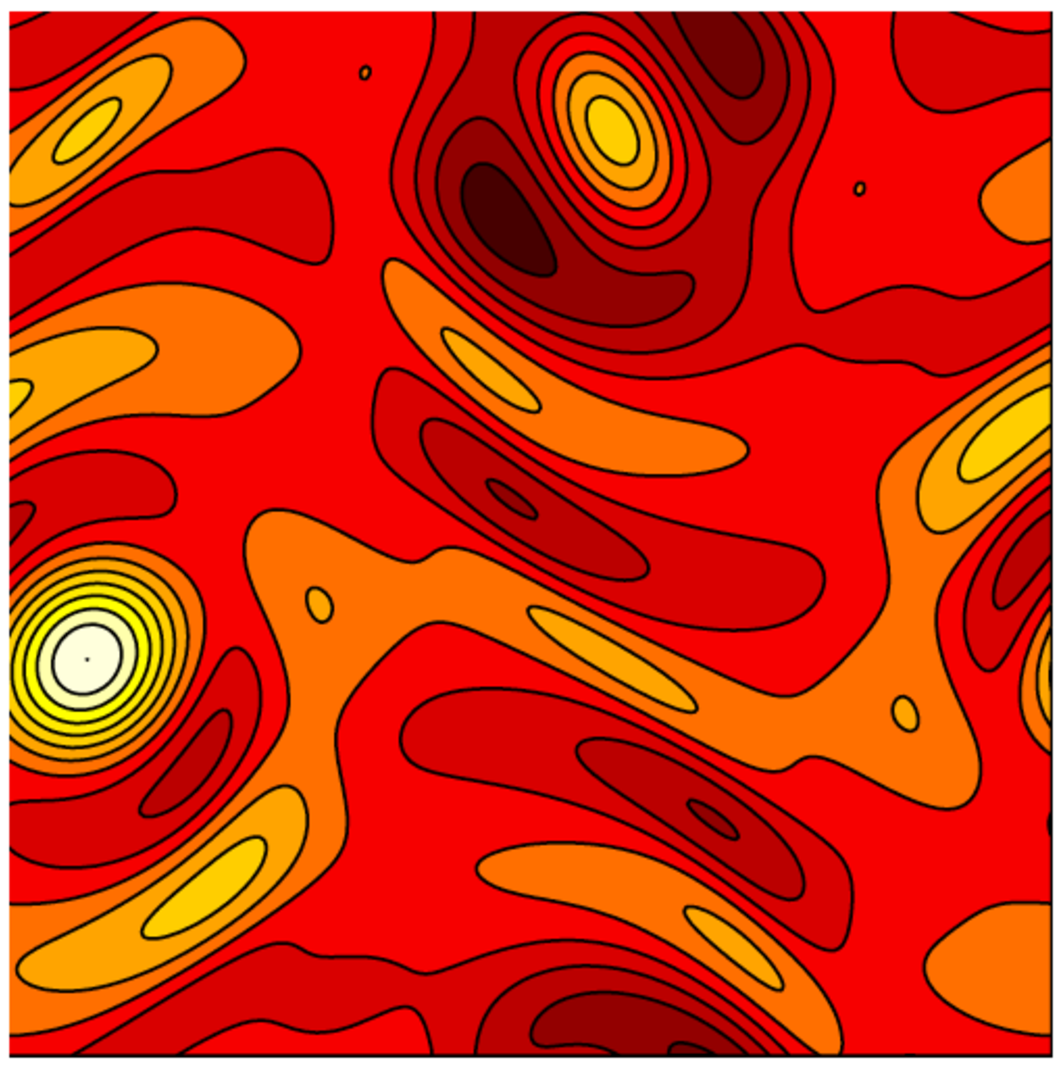
\includegraphics[width=.40\textwidth]{Kol_CK13_E1}
	(b)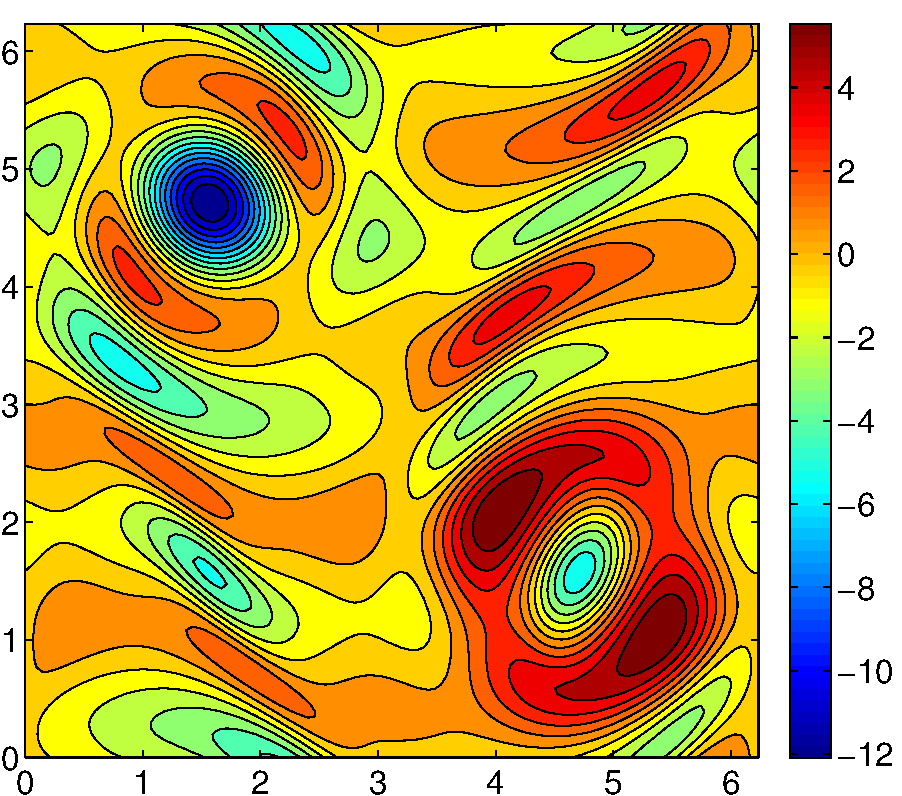
\includegraphics[width=.47\textwidth]{Kol_R40_n128_vort_adj+newton}
	\caption{(a) Equilibrium E1 found by Chandler \& Kerswell, JFM 722 (2013) (b) The
	same equilibrium found by adjoint equation integrated for $4\times 10^4$ time units
	(takes approximately $3$ minutes) plus 7 iterations of Newton-GMRES to decrease the
	$L^2$ error to $5\times 10^{-13}$. Here, $\mbox{Re}=40$. Note that panels (a) and (b)
	appear to be related
	by a shift-and-reflect symmetry.}
	\label{fig:Kol_R40_E1}
\end{figure}
}
	
\PCpost{2015-06-20}{
The Kolmogorov flow domain $(x,y)\in [0,2\pi]\times [0,2\pi]$ in
\refeq{eq:kolmogorov} really bugs me. The Rayleigh number controls the
viscosity legth scale, as compared to the strip width. Experimentally one
fixes the number $n$ of spanwise strips, and can chose any streamwise
length, so the domain should be a rectangle, such that for given $n$ and
$Re$ if one doubles the streamwise length, on doubles the number of
vortices, while keeping their shape intact. Forcing them  into a square
domain would squash the vortices. 3rd floor people must have thought all
this through...
}

\MFpost{2015-06-19}{Define the projection operator
\beq
\mathcal P\mathbf u = \frac{1}{4n}\sum_{m=0}^{2n-1}\mathcal
S^m\left[\mathbf u +\mathcal R\mathbf u\right],
\ee{MMFaxis1}
as the average over all discrete symmetries of the Kolmogorov flow
in the \slice. Let
$I[\mathbf u]$ denote the energy input for the state $\mathbf u$. For
Kolmogorov flow, the energy input $I[\mathbf u]$ is linear in $\mathbf
u$. Due to its linearity and since the energy input is conserved under
any symmetry action, we have $I[\mathcal P\mathbf u]=I[\mathbf u]$.
Therefore, $$I[\mathbf u-\mathcal P\mathbf u]=0,$$ that is all the
contribution to the energy input comes solely from the projection
$\mathcal P\mathbf u$!
}

\PCpost{2018-12-07}{
Blah blah.
}

\subsection{Kolmogorov Flow doubly periodic formulation}

The equations governing two dimensional Kolmogorov flow can be written in terms
of velocity field $\mathbf{u}$(eliminated later) and vorticity $\omega$ in the
following manner. For now I will just write the homogeneous equations, with
forcing easily added afterwards

\beq
\omega_t - \hat{z}\cdot(\nabla \times (\mathbf{u}\times \omega \hat{z})) - \frac{1}{Re}\nabla^2 \omega = 0
\eeq

The only difficult part of rewriting this equation in terms of $(2+1)$ spatiotemporal Fourier coefficients
(assuming periodic boundary conditions) is the nonlinear term, not only due to the cross products
but the necessity to express the velocity field in terms of the streamfunction, and consequently the
vorticity field as $\mathbf{u} = \nabla \times (\nabla^{-2} \omega)$
which is possible due to the two dimensional approximation. The operator $\nabla^{-2}$ is the inverse
of the Laplacian, which is technically singular; I asked around and the standard practice is to essentially
define it in fourier space as $\frac{1}{|\mathbf{k}|^2}$, where $|\mathbf{k}|^2 = k_x^2 + k_y^2$. For
numerical purposes its apparently common practice to say that the inverse of the $k_x = k_y = 0 $
term equals $1$. In other words, $1/0 = 1$. It's just a means of approximating the operator in
spectral space.

Although \rf{ChaKer12} give nice formula that is almost entirely of Fourier coefficients, I find it
more useful to completely eliminate the velocity field components $\mathbf{u} = (u,v)$ from the equation.

Therefore, the pseudospectral (homogeneous) spatiotemporal equation takes the form,

\bea \label{eqn:2DK_spectral}
\ii \omega \Omega &+& \ii k_x \mathcal{F}[\mathcal{F}^{-1}(\frac{\ii k_y}{|\mathbf{k}|^2} \Omega)* \mathcal{F}^{-1}(\Omega)] \continue
                  &-& \ii k_y \mathcal{F}[\mathcal{F}^{-1}(\frac{\ii k_x}{|\mathbf{k}|^2} \Omega)*\mathcal{F}^{-1}(\Omega)] \continue
                  &-& \frac{|\mathbf{k}|^2}{Re} \Omega = G(\Omega,T,L_x,L_y) = 0
\eea

Likewise, if allowed to write differentiation operators via $D_t,D_x,D_y$, etc, then the jacobian
takes on the form in pseudospectral representation,

\bea \label{eqn:2DK_spectral_jac}
J   &=& D_t + D_x \mathcal{F}[diag(D_y \nabla^{-2} \omega)\mathcal{F}^{-1} + diag(\omega)D_y \nabla^{-2}\mathcal{F}^{-1}]\continue
    &-& D_y \mathcal{F}[diag(D_x \nabla^{-2} \omega)\mathcal{F}^{-1} + diag(\omega)D_x \nabla^{-2}\mathcal{F}^{-1}] \continue
    &-& \frac{\nabla^2}{Re}
\eea

By taking the complex conjugate and multiplying by the Feynman equation \refeq{eqn:2DK_spectral},
the expression for the adjoint descent direction, $-J^{\dagger}G$.

\bea \label{eqn:2DK_adjointdescent}
-J^{\dagger}G  &=& [D_t + \mathcal{F}diag(D_y \nabla^{-2} \omega)\mathcal{F}^{-1} D_x \continue
               &-& \mathcal{F} \nabla^{-2} D_y diag(\omega)\mathcal{F}^{-1}D_x \continue
               &-& \mathcal{F}diag(D_x \nabla^{-2}\omega)\mathcal{F}^{-1} D_y\continue
               &+& \mathcal{F} \nabla^{-2} D_x diag(\omega)\mathcal{F}^{-1}D_y \continue
               &-& \frac{\nabla^2}{Re}] \cdot G
\eea

\subsection{Kolmogorov Flow non periodic boundary conditions}

Mike Schatz and I had a conversation today via Hangouts because he wanted
to follow up on our presentation and discuss how this could possibly be relevant
to his group. The main goal we discussed was to pursue a spatiotemporal numerical
formulation for a experimentally comparable setting, namely Kolmogorov flow without
doubly periodic boundary conditions and incorporating Rayleigh
friction. I explained that the key difference would
be to change to a Chebyshev polynomial basis due to the boundary conditions but work
with the vorticity field as is common practice.

For starters, I'll describe the basic formulation for \eqva\, in a Chebyshev-Chebyshev basis. The key details is that to have accurate or
viable numerics the spatial grid would have to be defined not on an equidistant,
rectangular grid but rather defined at (this is a specific choice, but a common one)
what are known as the Chebyshev-Gauss Lobatto quadrature nodes. In other words, any
initial condition would either have to be either initialized in spectral space (very very preferable), or initialized on the discretized grid defined by the set of points in physical space,

\beq \label{eqn:CGLnodes}
(x_m,y_n) = (\cos (\frac{\pi m }{M}),\cos (\frac{\pi n }{N}) \,.
\eeq

It is this discretization that allows us to use a (Chebyshev) polynomial basis
in a collocation method, as an equally spaced grid would induce error from
the Runge phenomenon (like the Gibbs phenomenon for Fourier modes but for polynomial bases). One benefit (I believe?) is that the discretization has a higher
resolution near the walls. Another benefit of this specific choice of quadrature nodes
is that by definition they are the points at which the derivative of the Chebyshev
polynomials are zero, \ie $T'(x_m) = 0$. Other choices, such as the Chebyshev-Gauss nodes would instead provide the condition $T(x_m) = 0$.

With a two-dimensional spatial grid defined on the Chebyshev-Gauss-Lobatto nodes,
we can use a discrete cosine transform to determine the spectral coefficients of the
Chebyshev polynomial basis \rf{CHQZ06}.

For a scalar vorticity field, $\omega(x_m,y_n)$, the corresponding Chebyshev modes
are calculated with the following formula

\beq
\Omega_{jk} = \frac{2}{M*N}\frac{1}{\bar{c}_j \bar{c}_k} \sum_{n,m} \frac{\omega_{nm}}{\bar{c}_n\bar{c}_m} \cos (\frac{\pi m j}{M})\cos (\frac{\pi n k}{N})
\eeq

and the corresponding inverse transformation given by

\beq
\omega_{nm}\Omega_{jk} = \sum_{j,k} \Omega_{jk} \cos (\frac{\pi m j}{M})\cos(\frac{\pi n k}{N}) \,.
\eeq

In this context there are no continuous translation symmetries, nor does the shit-reflect exist. The only remaining symmetry is in fact the rotational symmetry,
defined by action on the vorticity field $ R \cdot \omega (x,y) \rightarrow \omega (-x,-y)$.

Via the invariance condition,
\beq
\omega - R \cdot \omega = 0 \,,
\eeq
one can derive selection rules for the Chebyshev modes with spatial rotation symmetry. The rotation action is equivalent to the coordinate
transformation $x\rightarrow -x, y\rightarrow y$. Via the Chebyshev-Gauss-Lobatto relation,

\bea
x_m &=& \cos(\pi m / M) \continue
-x_m &=& -\cos(\pi m / M) \continue
-x_m &=& \cos(\pi)\cos(\pi m / M) \continue
-x_m &=& \cos(\pi m / M + \pi) \continue
\cos^{-1}(x_m) &=& \pi m / M  + \pi \continue
\eea

which after substitution into the invariance condition (in terms of Chebyshev modes),

\beq
\sum_{j,k}\Omega_{jk}\cos (\frac{\pi m j}{M})\cos(\frac{\pi n k}{N})
=\sum_{j,k}\Omega_{jk}\cos (\frac{\pi m j}{M}+j\pi)\cos(\frac{\pi n k}{N} + k\pi) \,,
\eeq

in turn implies the following,

\beq
\Omega_{jk} = (-1)^{j+k}\Omega_{jk} \mbox{for all} j,k.
\eeq

Therefore the subset of modes $(\Omega_{jk} : j+k = \mbox{odd})$ are forced
to be zero by discrete symmetry.

These selection rules hold only for solutions in the rotationally invariant subspace, naturally.





\end{description}

%%%%%%%%%%%%%%%%%%%%%%%%%%%%%%%%%%%%%%%%%%%%%%%%%%%%%%%%%%%%%%%%%%%%%%%
\printbibliography[heading=subbibintoc,title={References}]
